\chapter{Results}

Application is evolving from list, edit students and groups, to its final goals. These objectives were fulfilled:
\section{Objectives completed}
\begin{itemize}
  \item Access to any workday, any group and student.
  \item Management of attendance and misbehaviour of each student. The students information is still hard-coded into source files.
  \item 
\end{itemize}


\section{Technical details}
Javascript-SQL conexion
Asynchronous methods


\section{Further objectives}

\begin{itemize}
\item Links to student and group management. These pages were done but links are not missing into main application window.
\item There are several objectives not fulfilled yet, but I am on the way to get those done, those are, in priority order:
\item Data visualization. Student attendance and misbehaviour have to be shown in table-like window.
\item Test into real hardware. EduXes.apk has to be copied into mobile phone.
\item Activities evaluation per student. A window to display activities marks and final mark.
\item Timetable management. A window to manage groups timetable. When a group has class with this teacher.
\item Server synchronization with a custom application or

\end{itemize}

%%Como se desenvolveu o teu traballo, que obxectivos
%%> puideches acadar e cales non e porqu�. Inclu�r neste apartado a
%%> descrici�n da aplicaci�n desenvolvida, que � o que agora mesmo t�s no
%%> cap�tulo 4.Description.

These objectives were not fulfilled because time and skills lack.



En este apartado deber�n quedar reflejados los experimentos
realizados. Para ello se mostrar�n:
%% \cite{Cita}
\ref{fig:siestta30}
%% TODO: Screenshots:
\begin{figure}
    \begin{center}
        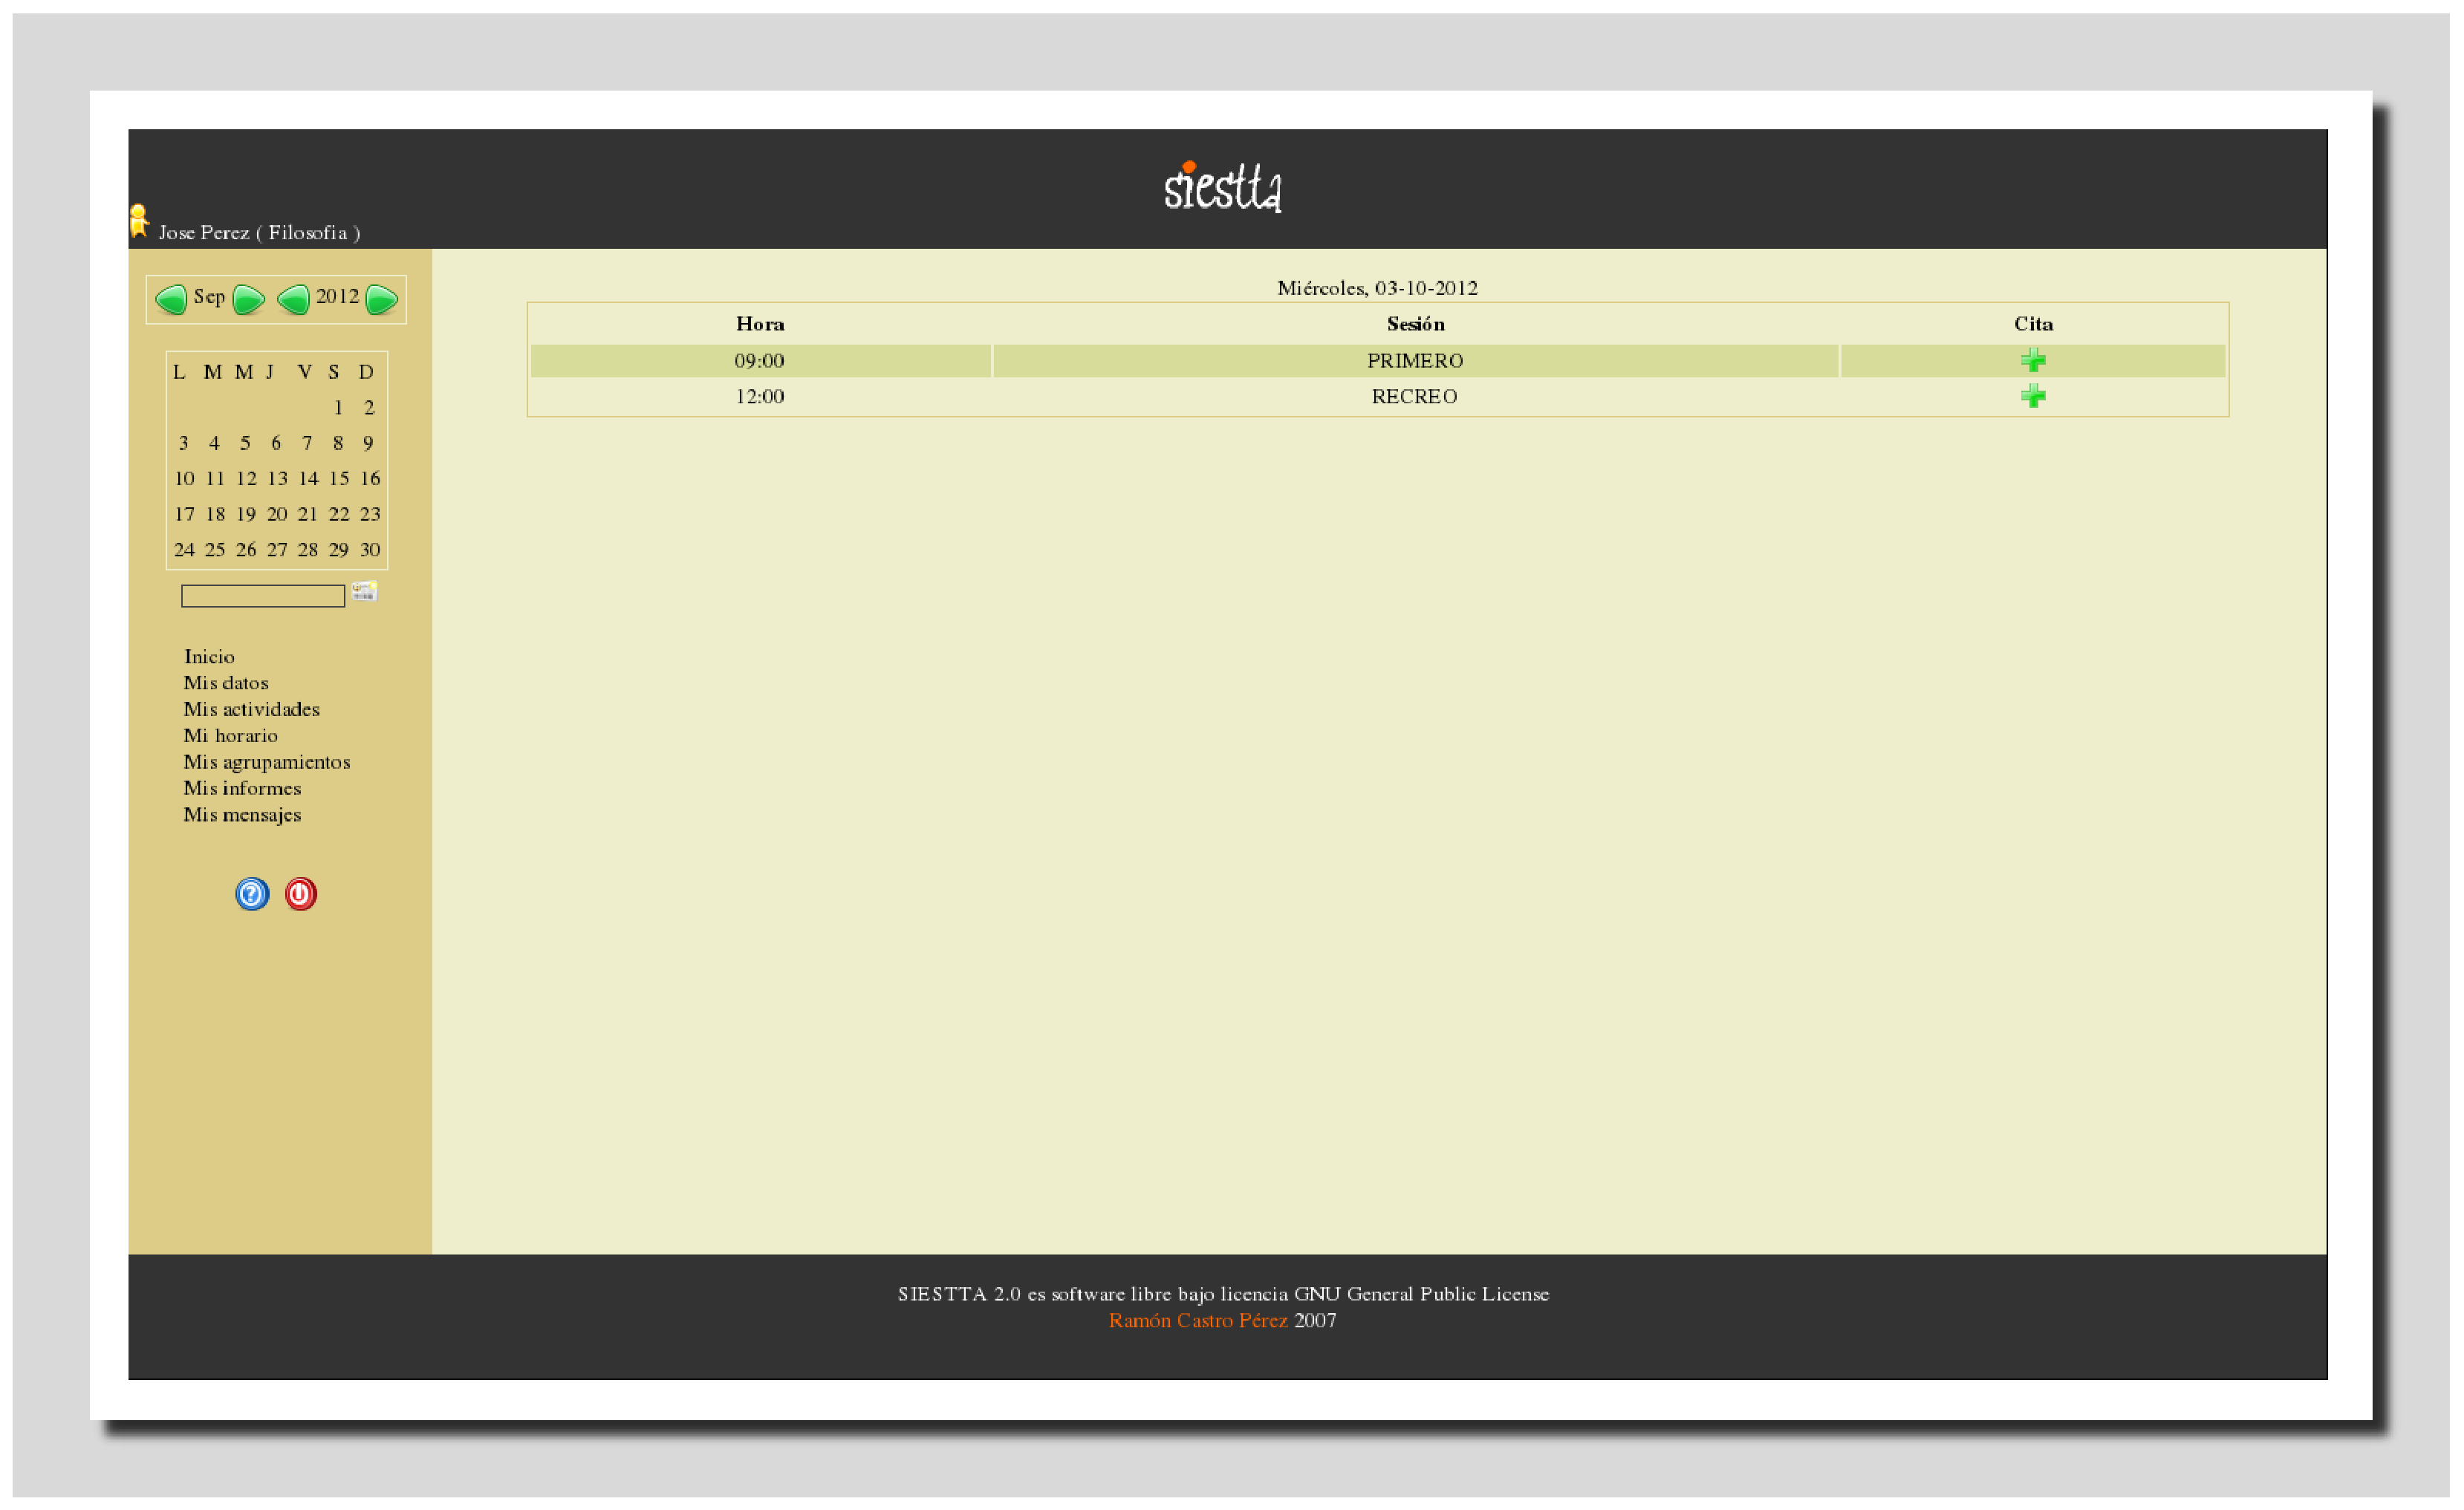
\includegraphics[width=\textwidth]{siestta2.eps}
        \caption{Siestta Main Page}
        \label{fig:siestta30}
    \end{center}
\end{figure}





\section {Resultados en forma de tablas, gr�ficas e im�genes donde se describa cuantitativa
            y cualitativamente el funcionamiento de la aplicaci�n} \dots

\section {An�lisis cr�tico de los resultados con el objetivo de decidir si el sistema implementado es v�lido}
\dots

Several problems were faced:
Eclipse environment: A stable, reliable and up-to-date IDE, with several plug-ins is needed. Download vanilla Eclipse Juno from its web-site is chosen because it is more stable, reliable, compatible with newer versions.  Aptana Javascript plugin was chosen because Aptana allows source code auto-completion in JQuery.
PhoneGap and Android incompatibilities. Android 2.3.3 requires JQuery-1.8.1 and does not work on higher versions. 
Error handlers. I have had several problems with tx.executeSql(...) function, it confused me with db.transaction(...): 
tx.executeSql(sql, [parameters],  successHandler, errorHandler)
and
db.transaction(queryFunction, errorHandler, successHandler)  
have up to four and three parameters respectively, only first one is mandatory. I rather use success and error handlers for tx.executeSql function, atomic error control could be better choice.
Passing variables to functions: Only if another solution is not known or feasible, global variables are used: named after global\_\*, and in block capitals.
Deadline. Development was delayed because I have no enough spare time and above problems were time costly.

\begin{verbatim}
 ohcount -i  assets/www/js/database.js assets/www/js/interface.js \
 assets/www/js/create_populate_db.js  assets/www/index.html \
 assets/www/remove.html 
Examining 5 file(s)
                              Ohloh Line Count                              
Language               Code    Comment  Comment %      Blank      Total  File
----------------  ---------  ---------  ---------  ---------  ---------  -----------------------------------------------
javascript             1374        155      10.1%        210       1739  database.js
javascript              393         91      18.8%         56        540  interface.js
javascript              402         57      12.4%         46        505  create_populate_db.js
html                    546         99      15.3%        117        762  index.html
javascript                1          0       0.0%          0          1  index.html
html                     28          1       3.4%          8         37  remove.html

\end{verbatim}
